\question ¿Cuánto pesaría una persona de 70 kg de masa si estuviera sobre la superficie de otros cuerpos celestes? Escribe en cada recuadro el valor de acuerdo con cada cuerpo celeste.

% \begin{tabular}{cc}
\begin{parts}
    \part[5]
    \begin{minipage}[t][][b]{0.2\textwidth}
        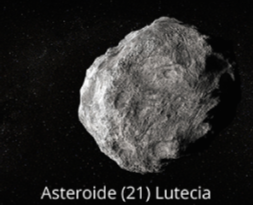
\includegraphics[width=\linewidth]{lutecia}
    \end{minipage}\hfill
    \begin{minipage}[c][][c]{0.5\textwidth}
        $g=0.05  m/s^2$   \fillin[] N
    \end{minipage}

    \part[5]
    \begin{minipage}[t][][b]{0.2\textwidth}
        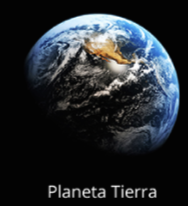
\includegraphics[width=\linewidth]{tierra}
    \end{minipage}\hfill
    \begin{minipage}[c][][c]{0.5\textwidth}
        $g=9.81  m/s^2$   \fillin[] N
    \end{minipage}

    \part[5]
    \begin{minipage}[t][][b]{0.2\textwidth}
        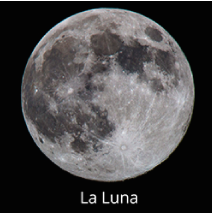
\includegraphics[width=\linewidth]{luna}
    \end{minipage}\hfill
    \begin{minipage}[c][][c]{0.5\textwidth}
        $g=1.62  m/s^2$   \fillin[] N
    \end{minipage}

    \part[5]
    \begin{minipage}[t][][b]{0.2\textwidth}
        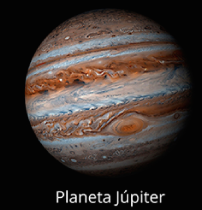
\includegraphics[width=\linewidth]{jupiter}
    \end{minipage}\hfill
    \begin{minipage}[c][][c]{0.5\textwidth}
        $g=24.79 m/s^2$   \fillin[] N
    \end{minipage}

\end{parts}
% \end{tabular}
